%------------------------
% Resume Template
% Author : Anubhav Singh
% Github : https://github.com/xprilion
% License : MIT
%------------------------

\documentclass[a4paper,20pt]{article}

\usepackage{latexsym}
\usepackage[empty]{fullpage}
\usepackage{titlesec}
\usepackage{marvosym}
\usepackage[usenames,dvipsnames]{color}
\usepackage{verbatim}
\usepackage{enumitem}
\usepackage[pdftex]{hyperref}
\usepackage{fancyhdr}
\usepackage{gensymb}
\usepackage{pdfpages} 

\pagestyle{fancy}
\fancyhf{} % clear all header and footer fields
\fancyfoot{}
\renewcommand{\headrulewidth}{0pt}
\renewcommand{\footrulewidth}{0pt}

% Adjust margins
\addtolength{\oddsidemargin}{-0.530in}
\addtolength{\evensidemargin}{-0.375in}
\addtolength{\textwidth}{1in}
\addtolength{\topmargin}{-.45in}
\addtolength{\textheight}{1in}

\urlstyle{rm}

\raggedbottom
\raggedright
\setlength{\tabcolsep}{0in}

% Sections formatting
\titleformat{\section}{
  \vspace{-10pt}\scshape\raggedright\large
}{}{0em}{}[\color{black}\titlerule \vspace{-6pt}]

%-------------------------
% Custom commands
\newcommand{\resumeItem}[2]{
  \item\small{
    \textbf{#1}{#2 \vspace{-2pt}}
  }
}

\newcommand{\resumeItemWithoutTitle}[1]{
  \item\small{
    {\vspace{-2pt}}
  }
}

\newcommand{\resumeSubheading}[4]{
  \vspace{-1pt}\item
    \begin{tabular*}{0.97\textwidth}{l@{\extracolsep{\fill}}r}
      \textbf{#1} & #2 \\
      \textit{#3} & \textit{#4} \\
    \end{tabular*}\vspace{-5pt}
}


\newcommand{\resumeSubItem}[2]{\resumeItem{#1}{#2}\vspace{-3pt}}

\renewcommand{\labelitemii}{$\circ$}

\newcommand{\resumeSubHeadingListStart}{\begin{itemize}[leftmargin=*]}
\newcommand{\resumeSubHeadingListEnd}{\end{itemize}}
\newcommand{\resumeItemListStart}{\begin{itemize}}
\newcommand{\resumeItemListEnd}{\end{itemize}\vspace{-5pt}}

%-----------------------------
%%%%%%  CV STARTS HERE  %%%%%%

\begin{document}

%----------HEADING-----------------
\begin{tabular*}{\textwidth}{l@{\extracolsep{\fill}}r}
  \textbf{{\LARGE Jeffrey Anderson}} & \href{mailto:jeffanderson867@ucla.edu}{jeffanderson867@ucla.edu} \\
  & 404-983-4994
  
  
\end{tabular*}
\vspace{-15pt}
%-----------EDUCATION-----------------
\section{Education}
  \resumeSubHeadingListStart
    \resumeSubheading
      {University of California - Los Angeles}{Los Angeles, CA}
      {Bachelor of Science - Mechanical Engineering - GPA: 3.54}{Expected Jun. 2022}
      {\scriptsize{ \footnotesize{\newline{}\textbf{Courses:} 
      Intermediate Fluid Mechanics, Advanced Strength of Materials, Principles of Nanoelectronics, Environmental Nanotechnology
      }}}
    \resumeSubHeadingListEnd
	    
\vspace{-10pt}

\section{Work Experience}
\resumeSubHeadingListStart
    \resumeSubheading{NanoClear Technology}{Pasadena, CA}
    {Process Engineer Associate}{May - Sep. 2019, Jun. - Dec. 2020}
    \resumeItemListStart
    	\resumeItem{}{Successful installation and validation of semiconductor process equipment including an e-beam evaporator and ICP etcher. Enlisted several contractors and developed standard operating procedures, recipes, and custom fixturing for unique substrates. Supporting documentation including standard operating procedures. }
    	\resumeItem{Substrate Dipping and Drying Robot}{: Developed a quick, low-cost, user programmable, and repeatable substrate dipping and drying robot on 3D printer platform. Led design review involving multiple disciplines. Supporting documentation.}
        \resumeItem{}
          {Custom tooling and supporting software for environmental materials testing of nano-enabled super-hydrophobic and super-hydophillic surfaces.
Custom chemical process hardware. Ported existing processes to new tooling and
applications. Enlisting prototyping manufacturers.}
	\resumeItem{Environmental Chamber}{: Environmental chamber for materials
testing. Involved Raspberry Pi, Arduino, PID control, and python application. Holds $\pm 0.5 \degree \textsc{C}$ and $-5\% \textsc{RH}$ with cycling behavior. Conducted design validation and presented supporting process data.}
    \resumeItemListEnd
    \resumeSubheading{California NanoSystems Institute - 
Integrated Systems Nanofabrication Cleanroom
}{Los Angeles, CA}
    {Lab Assistant}{Feb. - Jun. 2019}
    \resumeItemListStart
        \resumeItem{}
          {Ordering chemicals, ensuring tools operate within specifications, chemical waste handling, cleanroom specific tasks (particle count, laundry, etc.).
}
    \resumeItemListEnd
    \resumeSubheading{Wellstar Kennestone Hospital}{Marietta, GA}
    {Technician - Advanced Endoscopy Center and Linen Technician}{Jun. - Sep. 2018}
    \resumeItemListStart
        \resumeItem{}
          {Vital signs, patient transportation between rooms, room turnover, inventory, customer service, infection protocol and personal protective equipment
}
	\resumeItem{}{Distributing Linen }
    \resumeItemListEnd
    \resumeSubheading{Canister Design}{Woodstock, GA}
    {Software Development Intern}{Jun. - Jul. 2017}
    \resumeItemListStart
        \resumeItem{}
          {Introductory Swift IOS Development for MacOS and iOS applications, API interaction
}
    \resumeItemListEnd

\resumeSubHeadingListEnd

%-----------PROJECTS-----------------
\vspace{-10pt}
\section{Projects}
\resumeSubHeadingListStart
\resumeSubheading{University Cooperative Housing Association}{Los Angeles, CA}
	{Secretary of the Board of Directors} {Nov. 2020 - Pres.}
	\resumeItemListStart
		\resumeItem{}{Non-profit policy governance and COVID financial crisis management, providing affordable housing to over 400 student Angelenos. Team of seven elected directors and multiple committees.}
		\resumeItemListEnd
\resumeSubheading{Bruin Racing - Super Mileage}{Los Angeles, CA}
    {Powertrain Lead and Lab Manager}{Sep. 2018 - Pres.}
    \resumeItemListStart
    	\resumeItem{}{Project management of a six person team involving multiple disciplines, including mechanical and electrical design for torque sensing engine mount and belt driven starting mechanism supporting a high-efficiency vehicle.}
    	\resumeItem{}{Standard operating procedures and shop layout and organization.}
        \resumeItem{Torque Sensing Engine Mount}{: Sheet metal design for engine, wheel, and starter motor mounts.}
        \resumeItem{Fuel Pressurization}{: Pressure vessel and safe regulation for static fuel pressurization and 3D printed mounting hardware. Conducted design safety validation including burst testing.}
		\resumeItemListEnd
\vspace{-2pt}
\resumeSubItem{IdeaHacks2020 Hardware Hackathon, Education Category Winner}{: Automatic book reader using vision processing API on Raspberry Pi in under 48 hours. Five person team.}
		
\resumeSubItem{IdeaHacks2019 Hardware Hackathon, 1st Place Winner}{: RFID bike lock in under 48 hours using CAD, 3-D printers, and Arduino. Five person team.}


\vspace{2pt}
\resumeSubheading{UCLA Department of Mechanical and Aerospace Engineering}{Los Angeles, CA}
    {Student}{Sep. 2018 - Pres.}
    \resumeItemListStart
    	\resumeItem{2D Acoustic Mapper}{: Planer acoustic mapping using omnidirectional microphones and speaker.}
        \resumeItem{Engineering 96: Rockets}{: Carbon fiber and 3D printed model rockets(1-3 ft. in length). Suspended egg payload carrier.}
		\resumeItemListEnd
\vspace{2pt}
\resumeSubItem{For Fun}{: ESP32-based bluetooth keyboard(in progress). Raspberry Pi home VPN, network DNS ad blocking, and 3D printing server.}
\vspace{2pt}
\resumeSubHeadingListEnd

\vspace{-10pt}

\section{Skills Summary}
	\resumeSubHeadingListStart
	\resumeSubItem{Languages}{~~~~~~Python, MATLAB, Julia, \LaTeX, Arduino }
	\resumeSubItem{Tools}{~~~~~~~~~~~~~~SolidWorks, GIT, Minimal Simulink and KiCAD}
\resumeSubItem{OS}{~~~~~~~~~~~~~~~~~Linux(Manjaro, Ubuntu), Windows, MacOS}
\resumeSubHeadingListEnd

\vspace{-5pt}


%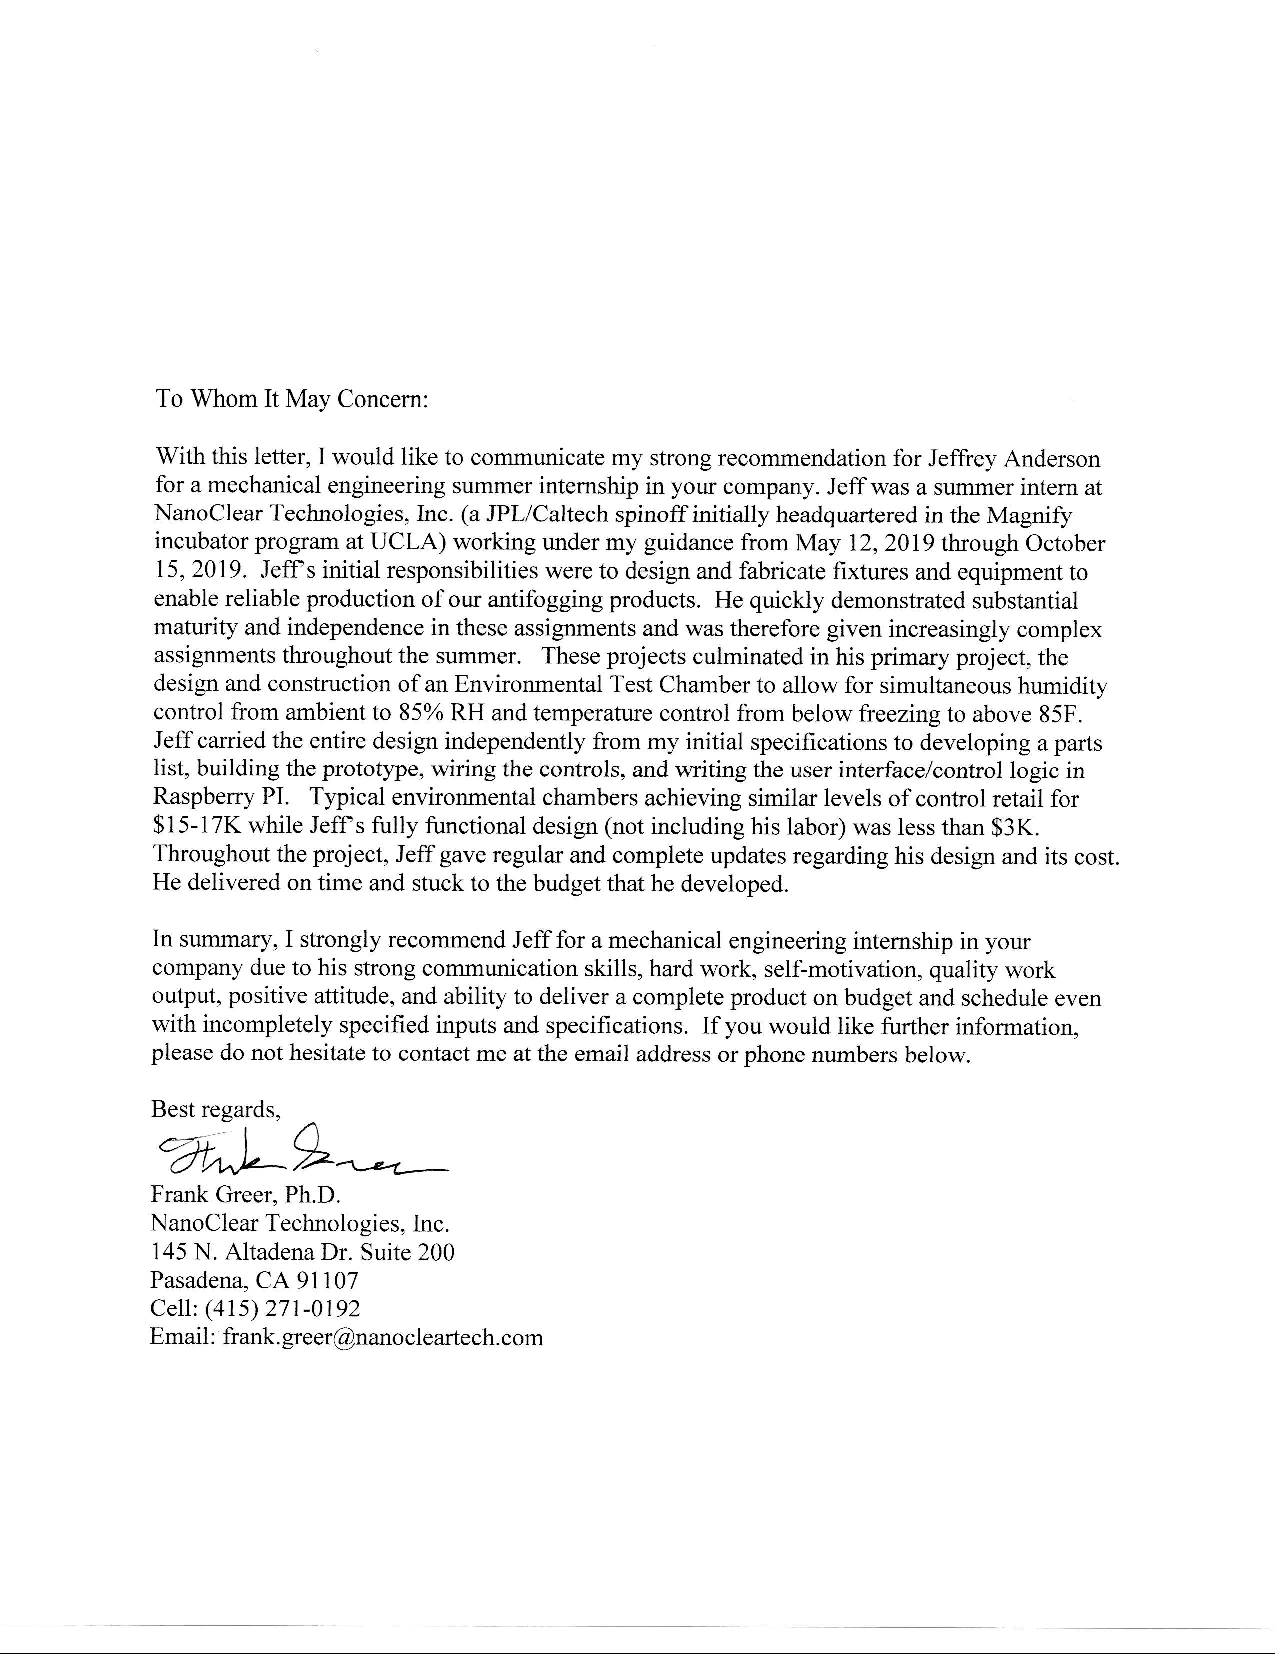
\includepdf[page={1}]{RecommendationLetter-FrankGreer}
\end{document}